\documentclass[12pt]{beamer}
\usepackage{../Estilos/BeamerMAF}
\usepackage{../Estilos/ColoresLatex}
\usetheme{Warsaw}
\usecolortheme{crane}
%\useoutertheme{default}
\setbeamercovered{invisible}
% or whatever (possibly just delete it)
\setbeamertemplate{section in toc}[sections numbered]
\setbeamertemplate{subsection in toc}[subsections numbered]
\setbeamertemplate{subsection in toc}{\leavevmode\leftskip=3.2em\rlap{\hskip-2em\inserttocsectionnumber.\inserttocsubsectionnumber}\inserttocsubsection\par}
\setbeamercolor{section in toc}{fg=blue}
\setbeamercolor{subsection in toc}{fg=blue}
\setbeamercolor{frametitle}{fg=blue}
\setbeamertemplate{caption}[numbered]

\setbeamertemplate{footline}
\beamertemplatenavigationsymbolsempty
\setbeamertemplate{headline}{}


\makeatletter
\setbeamercolor{section in foot}{bg=gray!30, fg=black!90!orange}
\setbeamercolor{subsection in foot}{bg=blue!30}
\setbeamercolor{date in foot}{bg=black}
\setbeamertemplate{footline}
{
  \leavevmode%
  \hbox{%
  \begin{beamercolorbox}[wd=.333333\paperwidth,ht=2.25ex,dp=1ex,center]{section in foot}%
    \usebeamerfont{section in foot} \insertsection
  \end{beamercolorbox}%
  \begin{beamercolorbox}[wd=.333333\paperwidth,ht=2.25ex,dp=1ex,center]{subsection in foot}%
    \usebeamerfont{subsection in foot}  \insertsubsection
  \end{beamercolorbox}%
  \begin{beamercolorbox}[wd=.333333\paperwidth,ht=2.25ex,dp=1ex,right]{date in head/foot}%
    \usebeamerfont{date in head/foot} \insertshortdate{} \hspace*{2em}
    \insertframenumber{} / \inserttotalframenumber \hspace*{2ex} 
  \end{beamercolorbox}}%
  \vskip0pt%
}
\makeatother

\makeatletter
\patchcmd{\beamer@sectionintoc}{\vskip1.5em}{\vskip0.8em}{}{}
\makeatother

\newlength{\depthofsumsign}
\setlength{\depthofsumsign}{\depthof{$\sum$}}
\newcommand{\nsum}[1][1.4]{% only for \displaystyle
    \mathop{%
        \raisebox
            {-#1\depthofsumsign+1\depthofsumsign}
            {\scalebox
                {#1}
                {$\displaystyle\sum$}%
            }
    }
}
\def\scaleint#1{\vcenter{\hbox{\scaleto[3ex]{\displaystyle\int}{#1}}}}
\def\scaleoint#1{\vcenter{\hbox{\scaleto[3ex]{\displaystyle\oint}{#1}}}}
\def\bs{\mkern-12mu}


\date{}

\title{\large{Ortogonalización de Gram-Schmidt}}
\subtitle{Tema 3 - Bases completas y ortogonales}
\author{M. en C. Gustavo Contreras Mayén}

\resetcounteronoverlays{saveenumi}

\begin{document}
\maketitle
\fontsize{14}{14}\selectfont
\spanishdecimal{.}

\section*{Contenido}
\frame{\tableofcontents[currentsection, hideallsubsections]}


\section{Ortogonalización de Gram-Schmidt}
\frame{\tableofcontents[currentsection, hideothersubsections]}
\subsection{Descripción}

\begin{frame}
\frametitle{El método de Gram-Schmidt}
Este método toma un conjunto de funciones (o vectores) no ortogonales linealmente dependientes y genera un conjunto ortogonal de funciones (o vectores) en un intervalo arbitrario con respecto a una función de peso arbitraria.
\end{frame}
\begin{frame}
\frametitle{El método de Gram-Schmidt}
Las funciones involucradas pueden ser reales o complejas, por conveniencia, asumiremos que las funciones son reales, la generalización para funciones complejas, no ofrece mayor dificultad.
\end{frame}
\begin{frame}
\frametitle{El método de Gram-Schmidt}
Veamos el caso de la normalización de funciones, que implica lo siguiente:
\pause
\begin{align*}
\scaleint{6ex}_{\bs a}^{b} \varphi_{i}^{2} \, w \, \dd{x}  =  N_{i}^{2}
\end{align*}
revisemos que no se le ha puesto atención al valor de $N_{i}$.
\end{frame}
\begin{frame}
\frametitle{El método de Gram-Schmidt}
Ya que la ecuación básica:
\pause
\begin{align}
\mathcal{L} \, u(x) + \lambda \, w(x) \, u(x) = 0
\label{eq:ecuacion_10_08}
\end{align}
es lineal y homogénea, podemos multiplicar la solución por cualquier constante, de tal manera que sigue siendo solución.
\end{frame}
\begin{frame}
\frametitle{El método de Gram-Schmidt}
Por lo que podemos pedir que tal solución $\varphi_{i}(x)$ se multiplique por $N_{i}^{-1}$ y ahora la nueva $\varphi_{i}$ (normalizada) $\varphi_{i}$ satisface:
\pause
\begin{align}
\scaleint{6ex}_{\bs a}^{b} \varphi_{i}^{2} (x) \, w(x) \, \dd{x} = 1
\label{eq:ecuacion_10_39}
\end{align}
\end{frame}
\begin{frame}
\frametitle{Funciones ortogonales y normalizadas}
En términos de una delta:
\pause
\begin{align}
\scaleint{6ex}_{\bs a}^{b} \varphi_{i}(x) , \varphi_{j} (x) \, w(x) \, \dd{x} = \delta_{ij}
\label{eq:ecuacion_10_40}
\end{align}
La ecuación (\ref{eq:ecuacion_10_39}) nos dice que hemos normalizado a la unidad; incluyendo la propiedad de ortogonalidad, tenemos la ecuación (\ref{eq:ecuacion_10_40}), las funciones que las satisfacen, se dice que son \textocolor{coolblack}{ortonormales} (ortogonales y normalizadas).
\end{frame}
\begin{frame}
\frametitle{Otro tipo de normalización}
Cabe señalar que existen otras formas de normalización, cada una de las funciones especiales de la Física Matemática se puede normalizar de distintas formas.
\end{frame}
\begin{frame}
\frametitle{Conjuntos de funciones}
Consideremos tres conjuntos de funciones:
\pause
\setbeamercolor{item projected}{bg=coolgrey,fg=black}
\setbeamertemplate{enumerate items}{%
\usebeamercolor[bg]{item projected}%
\raisebox{1.5pt}{\colorbox{bg}{\color{fg}\footnotesize\insertenumlabel}}%
}
\begin{enumerate}[<+->]
\item Un conjunto original, linealmente independiente $u_{n}(x)$ con $n = 0, 1 , 2 ,\ldots$. 
\\
Las funciones podrían ser funciones propias degeneradas, pero no es necesario que se cumpla este punto.
\item Un conjunto ortogonal $\psi_{n}(x)$ que se va a construir.
\item Un conjunto de funciones $\varphi_{n}(x)$ que será normalizadas $\psi_{n}(x)$
\end{enumerate}
\end{frame}
\begin{frame}
\frametitle{Propiedades de las funciones}
Tendremos las siguientes propiedades:
\pause
\begin{center}
{\fontsize{12}{12}\selectfont
\renewcommand{\arraystretch}{1.5}%
\begin{tabular}{p{2.7cm} p{2.7cm} p{2.7cm}}
\makecell{$u_{n}(x)$} & \makecell{$\psi_{n}(x)$} & \makecell{$\varphi_{n}(x)$} \\ \hline
\makecell{linealmente \\ independiente} &    \makecell{linealmente \\ independiente} & \makecell{linealmente \\ independiente} \\ \hline
\makecell{no ortogonal} & \makecell{ortogonal} & \makecell{ortogonal} \\ \hline
\makecell{no normalizada} & \makecell{no normalizada} & \makecell{normalizada \\ (ortonormal)} 
\end{tabular}
}
\end{center}
\end{frame}

\subsection{La técnica}

\begin{frame}
\frametitle{Procedimiento}
La técnica de Gram-Schmidt consiste en tomar la n-ésima función $\psi$ ($\psi_{n}$) para ser $u_{n}(x)$ más un combinación lineal no conocida de la función $\varphi$ previa.
\\
\bigskip
\pause
El que haya una nueva $u_{n}(x)$ nos dará la garantía de que se mantenga la independencia lineal.
\end{frame}
\begin{frame}
\frametitle{Procedimiento}
El que $\psi_{n}(x)$ sea ortogonal para cada una de las $\varphi$ previas, proporciona las suficientes restricciones para determinar los coeficientes desconocidos.
\\
\bigskip
\pause
Así cuando ya se determinen los $\psi_{n}$, se pueden normalizar a la unidad, dejando $\varphi_{n}(x)$. Este procedimiento se repite para las $\psi_{n+1}(x)$.
\end{frame}
\begin{frame}
\frametitle{Desarrollo de la técnica}
Empezamos con $n = 0$, sea:
\pause
\begin{align}
\psi_{0} = u_{0}(x)
\label{eq:ecuacion_10_41}
\end{align}
no nos preocupemos al no tener una $\varphi$ previa.
\\
\bigskip
\pause
Entonces normalizamos:
\pause
\begin{align}
\varphi_{0}(x) = \dfrac{\psi_{0}(x)}{\left[ \displaystyle \scaleint{6ex} \psi_{0}^{2} \, w \, \dd{x} \right]^{1/2}}
\label{eq:ecuacion_10_42}
\end{align}
\end{frame}
\begin{frame}
\frametitle{Desarrollo de la técnica}
Para $n = 1$, tenemos:
\pause
\begin{align}
\psi_{1}(x) = u_{1}(x) + a_{1,0} \, \varphi_{0}(x)
\label{eq:ecuacion_10_43}
\end{align}
\\
\bigskip
\pause
Que requiere que $\psi_{1}(x)$ sea ortogonal a $\varphi_{0}(x)$ (en este punto, la normalización de $\psi_{1}(x)$ es irrelevante).
\end{frame}
\begin{frame}
\frametitle{Desarrollo de la técnica}
La ortogonalidad nos conduce a:
\pause
\begin{align}
\begin{aligned}[b]
\scaleint{6ex} \psi_{1} \, \varphi_{0} \, w \, \dd{x} &= \scaleint{6ex} u_{1} \, \varphi_{0} \, w \, \dd{x} + \\
&+ a_{1,0} \scaleint{6ex} \varphi_{0}^{2} \, w \,  \dd{x} = 0
\end{aligned}
\label{eq:ecuacion_10_44}
\end{align}
\end{frame}
\begin{frame}
\frametitle{Desarrollo de la técnica}
Ya que $\varphi_{0}$ se normaliza a la unidad (ec. \ref{eq:ecuacion_10_42}), tenemos:
\pause
\begin{align}
a_{1,0} = - \scaleint{6ex} u_{1} \, \varphi_{0} \, w \, \dd{x}
\label{eq:ecuacion_10_45}
\end{align}
fijando el valor de $a_{1, 0}$.
\\
\bigskip
\pause
Normalizando, definimos:
\pause
\begin{align}
\varphi_{1} (x) = \dfrac{\psi_{1}(x)}{\left( \displaystyle \scaleint{6ex} \psi_{1}^{2} \, w \, \dd{x} \right)^{1/2}}
\label{eq:ecuacion_10_46}
\end{align}
\end{frame}
\begin{frame}
\frametitle{Desarrollo de la técnica}
Generalizando, resulta:
\pause
\begin{align}
\varphi_{i}(x) = \dfrac{\psi_{i}(x)}{\left( \displaystyle \scaleint{6ex} \psi_{i}^{2}(x) \, w(x) \, \dd{x} \right)^{1/2}}
\label{eq:ecuacion_10_47}
\end{align}
\\
\bigskip
\pause
donde:
\pause
\begin{align}
\psi_{i}(x) = u_{i} + a_{1, 0} \, \varphi_{0} + a_{i, 1} \, \varphi_{1} + \ldots + a_{i, i-1} \, \varphi_{i-1}
\label{eq:ecuacion_10_48}
\end{align}
\end{frame}
\begin{frame}
\frametitle{Desarrollo de la técnica}
Los coeficientes $a_{i, j}$ están dados por:
\pause
\begin{align}
a_{i, j} = - \scaleint{6ex} u_{i} \, \varphi_{j} \, w \, \dd{x}
\label{eq:ecuacion_10_49}
\end{align}
La ecuación (\ref{eq:ecuacion_10_49}) es para una normalización unitaria.
\\
\bigskip
\pause
Para otros tipos de normalización, se tiene que:
\pause
\begin{align*}
\scaleint{6ex}_{\bs a}^{b} \left[ \varphi_{j} (x) \right]^{2} \, w(x) \, \dd{x} =  N_{j}^{2}
\end{align*}
\end{frame}
\begin{frame}
\frametitle{Desarrollo de la técnica}
Entonces la ecuación (\ref{eq:ecuacion_10_47}) se reemplaza por:
\pause
\begin{align}
\varphi_{i}(x) =  N_{i} \: \dfrac{\psi_{i}(x)}{\left( \displaystyle \scaleint{6ex} \psi_{i}^{2} \, w \, \dd{x} \right)^{1/2}}
\label{eq:ecuacion_10_47a}
\end{align}
\\
\bigskip
\pause
y los términos $a_{i,j}$ resultan:
\pause
\begin{align}
a_{i, j} = - \dfrac{ \displaystyle \scaleint{6ex} u_{i} \, \varphi_{j} \, w \, \dd{x}}{N_{j}^{2}}
\label{eq:ecuacion_10_49a}
\end{align}
\end{frame}
\begin{frame}
\frametitle{Operadores de proyección}
Las ecuaciones (\ref{eq:ecuacion_10_48}) y (\ref{eq:ecuacion_10_49}) pueden escribirse en términos de operadores de proyección $P_{j}$.
\\
\bigskip
\pause
Si consideramos que $\varphi_{n}(x)$ forman un espacio vectorial lineal, la integral en la ecuación (\ref{eq:ecuacion_10_49}) puede interpretarse como la proyección de $u_{i}$ en la \enquote{coordenada} $\varphi_{j}$ o la componente $j$-ésima de $u_{i}$.
\end{frame}
\begin{frame}
\frametitle{Operadores de proyección}
Con:
\pause
\begin{align*}
P_{j} \, u_{i}(x) = \left[ \scaleint{6ex} u_{i}(t) \, \varphi_{j}(t) \, w(t) \dd{t} \right]\, \varphi_{j}(x)
\end{align*}
\pause
la ecuación (\ref{eq:ecuacion_10_48}) resulta ahora:
\pause
\begin{align}
\psi_{i}(x) = \left\{ 1 - \nsum_{j=1}^{i-1} P_{j} \right\} \, u_{i}(x)
\label{eq:ecuacion_10_48a}
\end{align}
\end{frame}
\begin{frame}
\frametitle{Operadores de proyección}
Restando los $j$-ésimos componentes: $j=1$ a $i-1$, resulta que $\psi_{i}(x)$ es ortogonal para todo $\varphi_{j}(x)$.
\\
\bigskip
\pause
Cabe señalar que el procedimiento de Gram-Schmidt es una manera de construir un conjunto ortogonal o ortonormal, pero las funciones $\varphi_{i}(x)$ no son únicas. \pause Existe un infinito de posibles conjuntos ortonormales para un intervalo dado y una función de peso dada.
\end{frame}

\subsection{Polinomios de Legendre}

\begin{frame}
\frametitle{Ejemplo Legendre}
Queremos generar un conjunto ortonormal a partir de las funciones:
\pause
\begin{align*}
u_{n}(x) = x^{n}, \hspace{1.5cm} n = 0, 1, 2, \ldots
\end{align*}
El intervalo es $-1 \leq x \leq 1$ y la función de peso es $w(x)=1$.
\end{frame}
\begin{frame}
\frametitle{Ejemplo Legendre}
De acuerdo a la técnica descrita de ortogonalización de Gram-Schmidt:
\pause
\begin{align}
u_{0} = 1 \hspace{1.5cm} \varphi_{0} =  \dfrac{1}{\sqrt{2}}
\label{eq:ecuacion_10_50}
\end{align}
\\
\bigskip
\pause
Entonces:
\pause
\begin{align}
\psi_{1}(x) = x + a_{1,0} \, \dfrac{1}{\sqrt{2}}
\label{eq:ecuacion_10_51}
\end{align}
\end{frame}
\begin{frame}
\frametitle{Ejemplo Legendre}
Donde:
\pause
\begin{align}
a_{1, 0} = - \scaleint{6ex}_{\bs -1}^{1} \dfrac{x}{\sqrt{2}} \, \dd{x} = 0
\label{eq:ecuacion_10_52}
\end{align}
por simetría.
\\
\bigskip
\pause
Normalizando $\psi_{1}$, obtenemos:
\pause
\begin{align}
\varphi_{1}(x) = \sqrt{\dfrac{3}{2}} \, x
\label{eq:ecuacion_10_53}
\end{align}
\end{frame}
\begin{frame}
\frametitle{Ejemplo Legendre}
Continuando el método de Gram-Schmidt, se define ahora:
\pause
\begin{align}
\psi_{2} (x) = x^{2} +  a_{2, 0} \, \dfrac{1}{\sqrt{2}} +  a_{2, 1} \, \sqrt{\dfrac{3}{2}} \, x
\label{eq:ecuacion_10_54}
\end{align}
\end{frame}
\begin{frame}
\frametitle{Ejemplo Legendre}
Donde:
\begin{align}
a_{2, 0} &= - \scaleint{6ex}_{\bs -1}^{1} \dfrac{x^{2}}{\sqrt{2}} \, \dd{x} = - \dfrac{\sqrt{2}}{3} \label{eq:ecuacion_10_55} \\[1em] 
a_{2, 1} &= - \scaleint{6ex}_{\bs -1}^{1} \sqrt{\dfrac{3}{2}} \, x^{3} \dd{x} = 0 \label{eq:ecuacion_10_56}
\end{align}
de nueva cuenta por simetría.
\end{frame}
\begin{frame}
\frametitle{Ejemplo Legendre}
Por tanto:
\pause
\begin{align}
\psi_{2}(x) = x^{2} - \dfrac{1}{3}
\label{eq:ecuacion_10_57}
\end{align}
\\
\bigskip
\pause
Normalizando a la unidad, tenemos:
\pause
\begin{align}
\varphi_{2} (x) = \sqrt{\dfrac{5}{2}} \, \dfrac{1}{2} \, (3 \, x^{2} - 1)
\label{eq:ecuacion_10_58}
\end{align}
\end{frame}
\begin{frame}
\frametitle{Ejemplo Legendre}
La siguiente función $\varphi_{3}(x)$ es:
\pause
\begin{align}
\varphi_{3} (x) = \sqrt{\dfrac{7}{2}} \, \dfrac{1}{2} \, (5 \, x^{3} - 3 \, x)
\label{eq:ecuacion_10_59}
\end{align}
\\
\bigskip
\pause
Se puede demostrar que:
\pause
\begin{align}
\varphi_{n}(x) = \sqrt{\dfrac{2 \, n + 1}{2}} \, P_{n}(x)
\label{eq:ecuacion_10_60}
\end{align}
donde $P_{n}$ es el polinomio de orden $n$ de Legendre.
\end{frame}

% \subsection{Ejercicio a cuenta}
\begin{frame}
\frametitle{Ejercicio a cuenta - 6}
Cuentas con los siguientes elementos:
\setbeamercolor{item projected}{bg=cornellred,fg=white}
\setbeamertemplate{enumerate items}{%
\usebeamercolor[bg]{item projected}%
\raisebox{1.5pt}{\colorbox{bg}{\color{fg}\footnotesize\insertenumlabel}}%
}
\begin{enumerate}[<+->]
\item Un conjunto de funciones $\left\{ u_{n} (x) \right\} = \left\{ x^{n} \right\}, \mbox{ con } n = 1, 2, \ldots$
\item El intervalo $(0, \infty)$
\item Una función de peso $w(x) = x \, e^{-x}$
\end{enumerate}
\end{frame}
\begin{frame}
\frametitle{Ejercicio a cuenta - 6}
Con el método de Gram-Schmidt construye las primeras \textbf{tres funciones ortonormales} del conjunto $u_{n}(x)$, con ese intervalo dado y función de peso dada.
\end{frame}


\section{Polinomios ortogonales}
\frame{\tableofcontents[currentsection, hideothersubsections]}
\subsection{Conjunto de polinomios}

\begin{frame}
\frametitle{Conjunto de funciones}
El ejemplo anterior se ha elegido estrictamente para ilustrar el procedimiento de Gram-Schmidt.
\\
\bigskip
\pause
Aunque tiene la ventaja de introducir los polinomios de Legendre, las funciones iniciales $u_{n} = x^{n}$ no son funciones propias degeneradas y no son soluciones de la ecuación de Legendre.
\end{frame}
\begin{frame}
\frametitle{Conjunto de funciones}
Son simplemente un conjunto de funciones que hemos reorganizado aquí para crear un conjunto ortonormal para el intervalo dado y la función de peso dada. 
\\
\bigskip
\pause
El hecho de que hayamos obtenido los polinomios de Legendre no es una magia negra, sino una consecuencia directa de la \textocolor{darkgreen}{elección de la función de peso y del intervalo}.
\end{frame}

% \begin{frame}[plain]
% %\frametitle{titulo}
% \fontsize{10}{10}\selectfont
% \begin{table}[!ht]
%     \centering
%     {\setlength\extrarowheight{1.5pt}
%     {\renewcommand{\arraystretch}{1.1}%
%     \begin{threeparttable}
%     \begin{tabular}{p{4cm} c c p{9cm}}
%     \hline
%     \makecell{Polinomios} & Intervalo & $w(x)$ & \makecell{Normalización estándar} \\ \hline
%     Legendre & $ -1 \leq x \leq 1$ & $1$ & $\displaystyle \int_{-1}^{1} \left[ P_{n}(x) \right]^{2} \dd{x} = \dfrac{2}{2 \, n + 1} $ \\
%     Modificados de Legendre & $ 0 \leq x \leq 1$ & $1$ & $\displaystyle \int_{-1}^{1} \left[ P_{n}^{*}(x) \right]^{2} \dd{x} = \dfrac{2}{2 \, n + 1} $ \\
%     Chebyshev I & $-1 \leq x \leq 1$ & $(1 - x^{2})^{-1/2}$ & $\displaystyle \int_{-1}^{1} \dfrac{\left[ T_{n}(x) \right]^{2}}{(1 - x^{2})^{-1/2}} \dd{x} = \begin{cases} 
%     \displaystyle \frac{\pi}{2} & n \neq 0 \\
%     \pi & n = 0 \end{cases} $ \\
%     Modificados de Chebyshev I & $0 \leq x \leq 1$ & $[x (1 - x)]^{-1/2}$ & $\displaystyle \int_{-1}^{1} \dfrac{\left[ T_{n}^{*} (x) \right]^{2}}{[x (1 - x)]^{-1/2}} \dd{x} = \begin{cases} 
%     \displaystyle \frac{\pi}{2} & n > 0 \\
%     \pi & n = 0 \end{cases} $ \\
%     Chebyshev II & $-1 \leq x \leq 1$ & $(1 - x^{2})^{1/2}$ & $\displaystyle\int_{-1}^{1} [U_{n} (x)]^{2} \, (1 - x^{2})^{1/2} \, \dd x = \frac{\pi}{2}$ \\
%     Laguerre & $0 \leq x < \infty $ & $e^{-x}$ & $\displaystyle \int_{0}^{\infty} \left[ L_{n} (x) \right]^{2} \, e^{-x} \dd{x} =  1 $ \\
%     Asociados de Laguerre & $0 \leq x < \infty $ & $x^{k} \, e^{-x}$ & $\displaystyle \int_{0}^{\infty} \left[ L_{n}^{k} (x) \right]^{2} \, x^{k} \, e^{-x} \dd{x} = \dfrac{(n + k)!}{n!} $ \\
%     Hermite & $- \infty < x < \infty $ & $e^{-x^{2}}$ & $\displaystyle \int_{-\infty}^{\infty} \left[ H_{n} (x) \right]^{2} e^{-x^{2}} \dd{x} = 2^{n} \, \pi^{1/2} \, n! $
%     \end{tabular}
%     \end{threeparttable}
%     }}
%     \end{table}
% \end{frame}
\begin{frame}
\frametitle{Elección de otras funciones e intervalos}
El uso de $u_{n} = x^{n}$ pero eligiendo otros intervalos y funciones de peso, nos conduce a otros conjuntos de polinomios ortogonales, como se muestra en la tabla (1):
\end{frame}
\begin{frame}[plain]
\frametitle{Tabla 1}
\begin{figure}
   \centering
   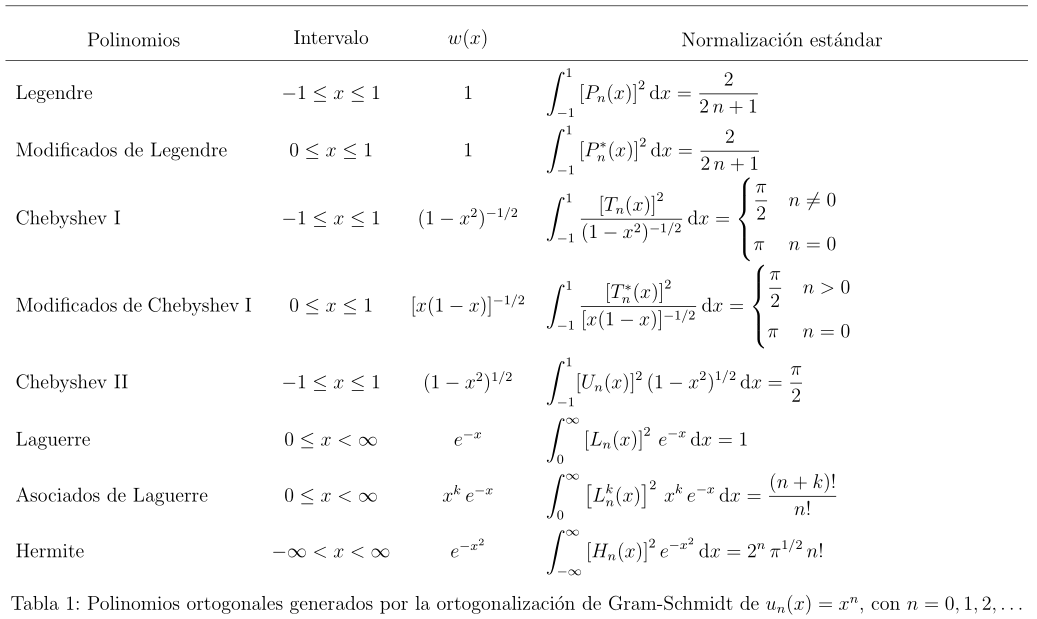
\includegraphics[scale=0.45]{Imagenes/Tabla_01.png}
\end{figure}
\end{frame}
% % \begin{landscape}
% % \begin{table}[H]
% % \centering
% % {\renewcommand{\arraystretch}{1.5}%
% % %\resizebox{\textwidth}{!}{%
% % \begin{tabular}{p{5cm} c c p{10cm}}
% % \hline
% % \makecell{Polinomios} & Intervalo & $w(x)$ & \makecell{Normalización estándar} \\ \hline
% % Legendre & $ -1 \leq x \leq 1$ & $1$ & $\displaystyle \scaleint{6ex}_{\bs -1}^{1} \left[ P_{n}(x) \right]^{2} \dd{x} = \dfrac{2}{2 \, n + 1} $ \\
% % Modificados de Legendre & $ 0 \leq x \leq 1$ & $1$ & $\displaystyle \scaleint{6ex}_{\bs -1}^{1} \left[ P_{n}^{*}(x) \right]^{2} \dd{x} = \dfrac{2}{2 \, n + 1} $ \\
% % Chebyshev I & $-1 \leq x \leq 1$ & $(1 - x^{2})^{-1/2}$ & $\displaystyle \scaleint{6ex}_{\bs -1}^{1} \dfrac{\left[ T_{n}(x) \right]^{2}}{(1 - x^{2})^{-1/2}} \dd{x} = \begin{cases} 
% % \displaystyle \frac{\pi}{2} & n \neq 0 \\
% % \pi & n = 0 \end{cases} $ \\
% % Modificados de Chebyshev I & $0 \leq x \leq 1$ & $[x (1 - x)]^{-1/2}$ & $\displaystyle \scaleint{6ex}_{\bs -1}^{1} \dfrac{\left[ T_{n}^{*} (x) \right]^{2}}{[x (1 - x)]^{-1/2}} \dd{x} = \begin{cases} 
% % \displaystyle \frac{\pi}{2} & n > 0 \\
% % \pi & n = 0 \end{cases} $ \\
% % Chebyshev II & $-1 \leq x \leq 1$ & $(1 - x^{2})^{1/2}$ & $\displaystyle\scaleint{6ex}_{\bs -1}^{1} [U_{n} (x)]^{2} \, (1 - x^{2})^{1/2} \, \dd x = \frac{\pi}{2}$ \\
% % Laguerre & $0 \leq x < \infty $ & $e^{-x}$ & $\displaystyle \scaleint{6ex}_{\bs 0}^{\infty} \left[ L_{n} (x) \right]^{2} \, e^{-x} \dd{x} =  1 $ \\
% % Asociados de Laguerre & $0 \leq x < \infty $ & $x^{k} \, e^{-x}$ & $\displaystyle \scaleint{6ex}_{\bs 0}^{\infty} \left[ L_{n}^{k} (x) \right]^{2} \, x^{k} \, e^{-x} \dd{x} = \dfrac{(n + k)!}{n!} $ \\
% % Hermite & $- \infty < x < \infty $ & $e^{-x^{2}}$ & $\displaystyle \scaleint{6ex}_{\bs -\infty}^{\infty} \left[ H_{n} (x) \right]^{2} e^{-x^{2}} \dd{x} = 2^{n} \, \pi^{1/2} \, n! $
% % \end{tabular}}
% % \caption{Polinomios ortogonales generados por la ortogonalización de Gram-Schmidt de $u_{n}(x)= x^{n}$, con $n=0,1,2,\ldots$}
% % \label{tabla:tabla_03}
% % \end{table}
% % \end{landscape}
\begin{frame}
\frametitle{La ortogonalización}
Una revisión de este proceso de ortogonalización revelará dos características arbitrarias:
\pause
\setbeamercolor{item projected}{bg=darkmagenta,fg=white}
\setbeamertemplate{enumerate items}{%
\usebeamercolor[bg]{item projected}%
\raisebox{1.5pt}{\colorbox{bg}{\color{fg}\footnotesize\insertenumlabel}}%
}
\begin{enumerate}[<+->]
\item Primero, como se enfatizó antes, no es necesario normalizar las funciones a la unidad.
En el ejemplo que acabamos de dar, podríamos haber requerido:
\pause
\begin{align}
\scaleint{6ex}_{\bs -1}^{1} \varphi_{n} (x) \: \varphi_{m} (x) \, \dd{x} = \dfrac{2}{2 \, n +1} \, \delta_{nm}
\label{eq:ecuacion_10_61}
\end{align}
y el conjunto resultante habría el de los polinomios de Legendre.
\seti
\end{enumerate}
\end{frame}
\begin{frame}
\frametitle{La ortogonalización}
\setbeamercolor{item projected}{bg=darkmagenta,fg=white}
\setbeamertemplate{enumerate items}{%
\usebeamercolor[bg]{item projected}%
\raisebox{1.5pt}{\colorbox{bg}{\color{fg}\footnotesize\insertenumlabel}}%
}
\begin{enumerate}[<+->]
\conti
\item Segundo, el signo de $\varphi_{n} (x)$ siempre es indeterminado.
\\
En el ejemplo, elegimos el signo al requerir que el coeficiente de mayor potencia de $x$ en el polinomio sea positivo. Para los polinomios de Laguerre, por otro lado, requeriríamos que el coeficiente de mayor potencia sea $(-1)^{n}/n!$
\end{enumerate}
\end{frame}

\section{Completes de las funciones propias}
\frame{\tableofcontents[currentsection, hideothersubsections]}
\subsection{Tercera propiedad}

\begin{frame}
\frametitle{Operador Hermitíano}
La tercera propiedad importante de un operador Hermitiano es que las funciones propias forman un conjunto completo. 
\end{frame}
\begin{frame}
\frametitle{¿Completez? Completitud?¿Cerradura?}
Como tal, el término \enquote{completes} es un tecnicismo, aunque aceptado pero no es correcto en español.
\\
\bigskip
\pause
Siendo la expresión \textocolor{darklava}{completitud} válida, mientras que \textocolor{darkscarlet}{compleción} es el término correcto, pero no es común encontrarla en los textos especializados tanto de matemática como de física en español. \pause En matemáticas es normal la referencia como \textocolor{darkviolet}{cerradura} o \enquote{clausura}.
\end{frame}
\begin{frame}
\frametitle{Propiedad operadores Hermitíanos}
Esta completes significa que cualquier función bien portada (al menos en partes pero continua) $F(x)$ se puede aproximar por una serie:
\pause
\begin{align}
F(x) = \nsum_{n=0}^{\infty} a_{n} \: \varphi_{n}(x) 
\label{eq:ecuacion_10_62}
\end{align}
con cualquier grado de precisión.
\end{frame}
\begin{frame}
\frametitle{Propiedad operador Hermitíano}
Con mayor formalismo, el conjunto $\varphi_{n} (x)$ se dice completo, si el límite del error medio cuadrado se anula:
\pause
\begin{align}
\lim_{m \to \infty} \scaleint{6ex}_{\bs a}^{b} \left[ F(x) - \nsum_{n=0}^{m} a_{n} \: \varphi_{n} \right]^{2} \, w(x) \, \dd{x} = 0
\label{eq:ecuacion_10_63}
\end{align}
\pause
Técnicamente, esta es una integral de Lebesgue. \pause No necesariamente el error es nulo en $[a,b]$, pero sólo la integral del error al cuadrado debe ser cero.
\end{frame}
\begin{frame}
\frametitle{Convergencia}
La convergencia en la media (ec. \ref{eq:ecuacion_10_63}) debe compararse con la convergencia uniforme.
\\
\bigskip
\pause
La convergencia uniforme implica la convergencia en la media, pero de manera inversa no se garantiza, la convergencia en la media es menos restrictiva.
\end{frame}
\begin{frame}
\frametitle{Cuando hay discontinuidades}
En la ecuación (\ref{eq:ecuacion_10_63}) no es válida para funciones continuas en piezas, ya que hay un número finito de discontinuidades.
\\
\bigskip
\pause
 En la ecuación (\ref{eq:ecuacion_10_62}) la expansión den los coeficientes $a_{m}$ se determina por:
\pause
\begin{align}
a_{m} = \scaleint{6ex}_{\bs a}^{b} F(x) \, \varphi_{m}^{*} (x) \, w(x) \, \dd{x}
\label{eq:ecuacion_10_64}
\end{align}
\pause
Que se obtiene al multiplicar la ecuación (\ref{eq:ecuacion_10_62}) por $\varphi_{m}^{*} \, w(x)$ y luego se integra.
\end{frame}
\begin{frame}
\frametitle{Presencia de la ortogonalidad}
De la ortogonalidad de las funciones propias $\varphi_{n}(x)$, solo el $m$-término sobrevive, por lo que la ortogonalidad es importante.
\\
\bigskip
\pause
La ecuación (\ref{eq:ecuacion_10_64}) puede compararse con el producto interno de vectores. En ocasiones los coeficientes $a_{m}$ son llamados \textbf{coeficientes generalizados de Fourier}.
\end{frame}
\begin{frame}
\frametitle{Integral definida}
Para una función conocida $F(x)$, la ecuación (\ref{eq:ecuacion_10_64}) devuelve $a_{m}$ como una \textbf{integral definida} que siempre se puede evaluar, ya sea numéricamente si es que no es de manera analítica.
\end{frame}
\begin{frame}
\frametitle{Espacio linealmente}
En términos del álgebra lineal, tenemos un espacio lineal, un espacio de funciones. 
\\
\bigskip
Las funciones linealmente independientes, ortonormales $\varphi_{n}(x)$ forman una base de ese espacio (infinito-dimensional).
\end{frame}
\begin{frame}
\frametitle{Espacio de Hilbert}
La ecuación (\ref{eq:ecuacion_10_62}) es un punto que nos dice que las funciones $\varphi_{n}(x)$ cubre ese espacio lineal.
\\
\bigskip
\pause
Con un producto punto definido por la ec. (\ref{eq:ecuacion_10_64}), el espacio lineal que tenemos, se convierte en un \textocolor{blue}{espacio de Hilbert}.
\end{frame}
\begin{frame}
\frametitle{Cerradura de un conjunto}
Por simplicidad, dejando la función de peso $w(x)=1$, la cerradura en forma de un operador para un conjunto discreto de eigenfunciones $\ket{\varphi_{i}}$ es:
\pause
\begin{align*}
\boxed{\nsum_{i} \ket{\varphi_{i}} \bra{\varphi_{i}} =  1}
\end{align*}
\end{frame}
\begin{frame}
\frametitle{Cerradura de un conjunto}
Multiplicando la relación de cerradura por $\ket{F}$. obtenemos la expansión de la eigenfunción:
\pause
\begin{align*}
\boxed{\ket{F} = \nsum_{i} \ket{\varphi_{i}} \braket{\varphi_{i}}{F}}
\end{align*}
con el coeficiente generalizado de Fourier $a_{i} = \braket{\varphi_{i}}{F}$.
\end{frame}
\begin{frame}
\frametitle{Representación coordenada}
De manera equivalente en una representación coordenada:
\pause
\begin{align*}
\boxed{\nsum_{i} \varphi_{i}^{*} (y) \: \varphi_{i} (x) = \delta (x - y)}
\end{align*}
\pause
implica que:
\pause
\begin{align*}
F(x) &= \scaleint{6ex} F(y) \: \delta (x {-} y) \, \dd{y} {=} \\
&= \nsum_{i} \varphi_{i} (x) \: \scaleint{6ex} \varphi_{i}^{*} (y) \: F(y) \dd{y}
\end{align*}
\end{frame}
% \begin{frame}
% \frametitle{Espectro de un operador}
% Sin pruebas, afirmamos que el espectro de un operador lineal $A$ que mapea un espacio de Hilbert $H$ en sí mismo puede dividirse en un espectro discreto (o puntual) con vectores propios de longitud finita, \pause un espectro continuo para que la ecuación de valores propios $A \, v = \lambda \, v$ con $v$ en $H$ no tiene una inversa limitada única $(A - \lambda)^{-1}$ en un dominio denso de $H$ y un espectro residual donde $(A - \lambda)^{-1}$.
% \end{frame}

\subsection{Desigualdad de Bessel}

\begin{frame}
\frametitle{Desigualdad de Bessel}
Si el conjunto de funciones $\varphi_{n} (x)$ no forma un conjunto completo, posiblemente sea por que no se han incluido el número infinito de elementos del conjunto completo, esto nos conduce a la \textocolor{red}{desigualdad de Bessel}. 
\end{frame}
\begin{frame}
\frametitle{Caso finito}
Consideremos primero un caso finito. Sea $\vb{A}$ un vector de $n$ componentes:
\pause
\begin{align}
\vb{A} = \vb{e}_{1} \, a_{1} + \vb{e}_{2} \, a_{2} + \ldots + \vb{e}_{n} \, a_{n} 
\label{eq:ecuacion_10_66}
\end{align}
en donde $\vb{e}_{i}$ es un vector unitario y $a_{i}$ es la correspondiente componente (proyección) de $\vb{A}$.
\end{frame}
\begin{frame}
\frametitle{Caso finito}
Esto es
\pause
\begin{align}
a_{i} = \vb{A} \cdot \vb{e}_{i}
\label{eq:ecuacion_10_67}
\end{align}
\pause
Entonces:
\pause
\begin{align}
\left( \vb{A} - \nsum_{i} \vb{e}_{i} \, a_{i} \right)^{2} \geq 0
\label{eq:ecuacion_10_68}
\end{align}
\end{frame}
\begin{frame}
\frametitle{Caso finito}
Si sumamos todos los $n$ componentes, la suma se iguala a $\vb{A}$ por lo que la ecuación (\ref{eq:ecuacion_10_66}) se mantiene, pero si la suma, no incluye a todos los $n$ componentes, la desigualdad se mantiene.
\\
\bigskip
\pause
Pero si la suma no incluye todos los $n$ componentes, se presenta la desigualdad.
\end{frame}
\begin{frame}
\frametitle{Caso finito}
Expandiendo la ecuación (\ref{eq:ecuacion_10_68}) y eligiendo los vectores unitarios para que satisfagan la relación de ortogonalidad:
\pause
\begin{align}
\vb{e}_{i} \cdot \vb{e}_{j} =  \delta_{ij}
\label{eq:ecuacion_10_69}
\end{align}
\pause
tenemos que:
\pause
\begin{align}:
\vb{A}^{2} \geq \nsum_{i} a_{i}^{2}
\label{eq:ecuacion_10_70}
\end{align}
Que es \underline{la desigualdad de Bessel}.
\end{frame}
\begin{frame}
\frametitle{Caso funciones reales}
Para funciones reales debemos de considerar la integral:
\pause
\begin{align}
\scaleint{6ex}_{\bs a}^{b} \left[ f(x) - \nsum_{i} a_{i} \: \varphi_{i}(x) \right]^{2} \, w(x) \, \dd{x} \geq 0
\label{eq:ecuacion_10_71}
\end{align}
\pause
que es el análogo continuo de la ecuación (\ref{eq:ecuacion_10_68}), haciendo $n \to \infty$ y reemplazando la suma por la integración. 
\end{frame}
\begin{frame}
\frametitle{Caso funciones reales}
Nuevamente, con el factor de peso $w(x) > 0 $, el integrando es no negativo.
\\
\bigskip
\pause
La integral se anula por la ecuación (\ref{eq:ecuacion_10_62}) si tenemos un conjunto completo. De otra forma, es positiva.
\end{frame}
\begin{frame}
\frametitle{Expansión de términos}
Si expandimos el término al cuadrado obtenemos:
\pause
\begin{align}
\begin{aligned}
&\scaleint{6ex}_{\bs a}^{b} [ f(x) ]^{2} \, w(x) \, \dd{x} + \\
&- 2 \nsum_{i} a_{i} \, \scaleint{6ex}_{\bs a}^{b} f(x) \, \varphi (x) \, w(x) \, \dd{x} + \\
+& \nsum_{i} a_{i}^{2} \geq 0
\end{aligned}
\label{eq:ecuacion_10_72}
\end{align}
\end{frame}
\begin{frame}
\frametitle{Expansión de términos}
Usando la ecuación (\ref{eq:ecuacion_10_64}), tenemos:
\pause
\begin{align}
\scaleint{6ex}_{\bs a}^{b} [f(x)]^{2} \, w(x) \, \dd{x} \geq \nsum_{i} a_{i}^{2}
\label{eq:ecuacion_10_73}
\end{align}
\end{frame}
\begin{frame}
\frametitle{Expansión de términos}
De aquí que la suma de los cuadrados de la expansión de los coeficientes $a_{i}$ es menor o igual que la integral de peso de $[f(x)]^{2}$, la igualdad se mantiene si y sólo si, la expansión es exacta, esto ocurre si el conjunto de soluciones $\varphi_{n}(x)$ es un conjunto completo.
\end{frame}
\begin{frame}
\frametitle{Uso de la desigualdad}
La desigualdad de Bessel tiene distintos usos, incluida la prueba de convergencia para las series de Fourier.
\end{frame}

\subsection{Desigualdad de Schwarz}

\begin{frame}
\frametitle{La desigualdad de Schwarz}
La desigualdad de Schwarz se usa comúnmente y es similar a la desigualdad de Bessel.
\\
\bigskip
\pause
Consideremos la ecuación cuadrática con la incógnita $x$:
\pause
\begin{align}
\nsum_{i=1}^{n} (a_{i} \, x + b_{i})^{2} = \nsum_{i=1}^{n} a_{i}^{2} \left( x + \frac{b_{i}}{a_{i}} \right)^{2} = 0
\label{eq:ecuacion_10_74}
\end{align}
Con $a_{i}$, $b_{i}$ reales.
\end{frame}
\begin{frame}
\frametitle{La desigualdad de Schwarz}
Si $b_{i}/a_{i}$ es la constante $c$, independiente del índice $i$, la solución es $x= - c$. 
\\
\bigskip
\pause
Si $b_{i}/a_{i}$ no es constante en $i$, todos los términos no se anulan simultáneamente para un $x$ real, por lo que la solución debe de ser compleja.
\end{frame}
\begin{frame}
\frametitle{Expansión de términos}
Expandiendo, tenemos que
\pause:
\begin{align}
x^{2} \, \nsum_{i}^{n} a_{i}^{2} + 2 \, x \, \nsum_{i}^{n} a_{i} \, b_{i} + \nsum_{i}^{n} b_{i}^{2} = 0
\label{eq:ecuacion_10_75}
\end{align}
\pause
como $x$ es complejo (o = $-b_{i}/a_{i}$)
\end{frame}
\begin{frame}
\frametitle{Expansión de términos}
La fórmula cuadrática para $x$ conduce a:
\pause
\begin{align}
\left( \nsum_{i=1}^{n} a_{i} \, b_{i} \right)^{2} \leq \left( \nsum_{i=1}^{n} a_{i}^{2} \right) \, \left( \nsum_{i=1}^{n} b_{i}^{2} \right)
\label{eq:ecuacion_10_76}
\end{align}
la igualdad se mantiene cuando $b_{i}/a_{i}$ es una constante independiente de $i$.
\end{frame}
\begin{frame}
\frametitle{Considerando vectores}
Nuevamente, en términos de vectores, tenemos:
\pause
\begin{align}
( \vb{a} \cdot \vb{b} )^{2} =  a^{2} \, b^{2} \, \cos^{2} \theta \leq a^{2} \, b^{2}
\label{eq:ecuacion_10_77}
\end{align}
donde $\theta$ es el ángulo entre $\vb{a}$ y $\vb{b}$.
\end{frame}
\begin{frame}
\frametitle{Caso con funciones complejas}
La desigualdad de Schwarz para funciones complejas tiene la expresión:
\pause
\begin{align}
\begin{aligned}
&\abs{ \scaleint{6ex}_{\bs a}^{b} f^{*} (x) \, g(x) \dd{x} }^{2} \leq \\
&\leq \scaleint{6ex}_{\bs a}^{b} f^{*}(x) \, f(x) \dd{x} \scaleint{6ex}_{\bs a}^{b} g^{*}(x) \, g(x) \dd{x}
\end{aligned}
\label{eq:ecuacion_10_78}
\end{align}
\end{frame}
\begin{frame}
\frametitle{Caso con funciones complejas}
La desigualdad se mantiene si y sólo si $g(x) = \alpha \, f(x)$, siendo $\alpha$ una constante.
% \\
% \bigskip
% \pause
% Para probar esta forma de la función de la desigualdad de Schwarz, consideremos la función compleja $\psi(x) = f(x) + \lambda \, g(x)$ con $\lambda$ una constante compleja, donde las funciones $f(x)$ y $g(x)$ son cualesquiera dos funciones de cuadrado integrable (para las cuales, las integrales del lado derecho existen).
\end{frame}
% \begin{frame}
% \frametitle{Caso con funciones complejas}
% Multiplicando por el conjugado complejo y luego integrando, tenemos:
% \pause
% \begin{align}
% \begin{aligned}
% \scaleint{6ex}_{\bs a}^{b} \psi^{*} \, \psi \, \dd{x} &\equiv \scaleint{6ex}_{\bs a}^{b} f^{*} \, f \dd{x} + \lambda \scaleint{6ex}_{\bs a}^{b} f^{*} \, g \dd{x} + \\
% &+ \lambda^{*} \scaleint{6ex}_{\bs a}^{b} g^{*} \, f \dd{x} + \\
% &+ \lambda \, \lambda^{*} \scaleint{6ex}_{\bs a}^{b} g^{*} \, g \dd{x}  \geq 0
% \end{aligned}
% \label{eq:ecuacion_10_79}
% \end{align}
% \end{frame}
% \begin{frame}
% \frametitle{Caso con funciones complejas}
% El $\geq 0$ aparece ya que $\psi^{*} \, \psi$ es no negativo, el signo igual $(=)$ se mantiene sólo si $\psi (x)$ es idéntico a cero. 
% \\
% \bigskip
% \pause
% Nótese que $\lambda$ y $\lambda^{*}$ son linealmente independientes, diferenciamos con respecto a uno de ellos, e igualamos la derivada a cero para minimizar:
% \pause
% \begin{align*}
% \scaleint{6ex}_{\bs a}^{b} \psi^{*} \, \psi \dd{x}
% \end{align*}
% \end{frame}
% \begin{frame}
% \frametitle{Caso con funciones complejas}
% \begin{align*}
% \pdv{\lambda^{*}} \scaleint{6ex}_{\bs a}^{b} \psi^{*} \, \psi \dd{x} = \scaleint{6ex}_{\bs a}^{b} g^{*} \, f \dd{x}  + \lambda \scaleint{6ex}_{\bs a}^{b} g^{*} g \dd{x} = 0
% \end{align*}
% \pause
% que nos da:
% \pause
% \begin{align}
% \lambda = - \dfrac{\displaystyle \scaleint{6ex}_{\bs a}^{b} g^{*} \, f \, \dd{x}}{\displaystyle \scaleint{6ex}_{\bs a}^{b} g^{*} \, g \, \dd{x}}
% \label{eq:ecuacion_10_80a}
% \end{align}
% \end{frame}
% \begin{frame}
% \frametitle{Caso con funciones complejas}
% Tomando el conjugado complejo:
% \pause
% \begin{align}
% \lambda^{*} = - \dfrac{\displaystyle \scaleint{6ex}_{\bs a}^{b} f^{*} \, g \, \dd{x}}{\displaystyle \scaleint{6ex}_{\bs a}^{b} g^{*} \, g \, \dd{x}}
% \label{eq:ecuacion_80b}
% \end{align}
% \pause
% sustituyendo esos valores de $\lambda$ y $\lambda^{*}$ en la ecuación (\ref{eq:ecuacion_10_79}), obtenemos la ecuación (\ref{eq:ecuacion_10_78}), \underline{la desigualdad de Schwarz}.
% \end{frame}
\begin{frame}
\frametitle{Ejemplos de uso}
En mecánica cuántica las funciones $f(x)$ y $g(x)$ podrían representar un estado o una configuración de un sistema físico, es decir, una combinación lineal de funciones de onda.
\end{frame}
\begin{frame}
\frametitle{Ejemplos de uso}
Entonces la desigualdad e Schwarz garantiza que el producto punto $\displaystyle \scaleint{6ex}_{\bs a}^{b} f^{*} \, g(x) \dd{x}$ existe. 
\\
\bigskip
\pause
En algunos textos, la desigualdad de Schwarz es un paso para llegar al principio de incertidumbre de Heinsenberg.
\end{frame}
% \begin{frame}
% \frametitle{Ejemplos de uso}
% La notación de las funciones de las ecuaciones (\ref{eq:ecuacion_10_78}) y (\ref{eq:ecuacion_10_79}) es a veces incómoda; en mecánica cuántica es común utilizar la notación de Dirac.
% \\
% \bigskip
% Con esta notación, se simplifica tanto el rango de integración $(a, b)$, como la función de peso $w(x) \geq 0$.
% \end{frame}
% \begin{frame}
% \frametitle{Ejemplos de uso}
% La desigualdad de Schwarz ahora se representa:
% \pause
% \begin{align}
% \abs{\braket{f}{g}}^{2} \leq \braket{f}{f} \, \braket{g}{g}
% \label{eq:ecuacion_10_78a}
% \end{align}
% \pause
% Si $g(x)$ es una función propia normalizada, $\varphi_{i}(x)$, la ecuación (\ref{eq:ecuacion_10_78}) lleva a (donde $w(x)=1$)
% \begin{align}
% a_{i}^{*} \, a_{i} \leq \scaleint{6ex}_{\bs a}^{b} f^{*}(x) \, f(x) \, \dd{x} 
% \label{eq:ecuacion_10_81}
% \end{align}
% Un resultado que se sigue de la ecuación (\ref{eq:ecuacion_10_73}).
% \end{frame}
% \subsection{Ejercicios a cuenta}
% \begin{frame}
% \frametitle{Ejercicio a cuenta}
% Demuestra que:
% \begin{align*}
% &\scaleint{6ex}_{\bs -\infty}^{\infty} \left( t^{10} - t^{6} + 5 \, t^{4} - 5 \right) \, e^{-4} \dd{t} \leq \\
% &\leq \sqrt{\scaleint{6ex}_{\bs -\infty}^{\infty} \left( t^{4} - 1 \right)^{2} \, e^{-4} \dd{t}} \, \sqrt{\scaleint{6ex}_{\bs -\infty}^{\infty} \left( t^{6} + 5 \right)^{2} \, e^{-4} \dd{t}}
% \end{align*}
% \end{frame}
% \begin{frame}
% \frametitle{Ejercicio a cuenta}
% Determina las funciones que satisfacen la ecuación de valores propios
% \begin{align*}
% \hat{A} \, f(x) = \lambda \, f(x)
% \end{align*}
% cuando $\hat{A}$ es el operador que al aplicarse a una función, la eleva al cuadrado.
% \end{frame}

\section{Ejercicio de normalización}
\frame{\tableofcontents[currentsection, hideothersubsections]}
\subsection{Enunciado}

\begin{frame}
\frametitle{Enunciado del problema}
Con el método de ortogonalización de Gram-Schmidt construye los primeros tres polinomios de Chebyshev de Tipo II.
\end{frame}
\begin{frame}
\frametitle{Elementos para el procedimiento}
Considera lo siguiente:
\pause
\begin{table}
\begin{tabular}{l l}
Funciones lineal. indep. & $u_{n}(x) = x^{n}$ \\
 & $n = 0, 1, 2, \ldots$ \\ \pause
Intervalo & $-1 \leq x \leq 1$ \\ \pause
Función de peso & $\omega (x) = (1 -x^{2})^{\frac{1}{2}}$
\end{tabular}
\end{table}
\end{frame}

\subsection{Normalización}

\begin{frame}
\frametitle{Normalización de los polinomios de Chebyshev}
La normalización de los polinomios de Chebyshev de tipo II $U_{n}(x)$, está dada por la expresión:
\pause
\begin{align*}
\scaleint{6ex}_{\bs \bs -1}^{1} \, U_{m}(x) \, U_{n} (x) \, \omega (x) \dd{x} = \delta_{mn} \, \dfrac{\pi}{2}
\end{align*}
\end{frame}
\begin{frame}
\frametitle{Normalización a considerar}
Dada la normalización de los $U_{n}$, hay que tomar en cuenta que:
\pause
\begin{eqnarray*}
&\scaleint{5ex}_{\bs a}^{b} \left[ \varphi_{j} (x) \right]^{2} \, \omega (x) \dd{x} = \\[0.5em] \pause
&\scaleint{6ex}_{\bs \bs -1}^{1} \, U_{m}(x) \, U_{n} (x) \, \omega (x) \dd{x} = \\[0.5em] \pause
&= \delta_{mn} \, \dfrac{\pi}{2} = \pause N_{j}^{2}
\end{eqnarray*}
\end{frame}
\begin{frame}
\frametitle{Expresión para normalizar}
Entonces tenemos que:
\pause
\begin{align*}
\varphi_{i} (x) =  N_{i} \: \dfrac{\psi_{i} (x)}{ \bigg[ \displaystyle \scaleint{5ex} \psi_{i}^{2} \, \omega \dd{x} \bigg]^{1/2}}
\end{align*}
\end{frame}
\begin{frame}
\frametitle{Los términos $a_{i,j}$}
Los términos $a_{i,j}$ resultan:
\pause
\begin{align}
a_{i, j} = - \dfrac{ \displaystyle \scaleint{5ex} u_{i} \, \varphi_{j} \, \omega \dd{x}}{N_{j}^{2}}
\label{eq:ecuacion_10_49a2}
\end{align}
\end{frame}    

\subsection*{Integral de apoyo}

\begin{frame}
\frametitle{Integral de apoyo}
Para reducir el tiempo en el cálculo de algunas integrales, nos apoyaremos con el siguiente resultado:
\pause
\begin{align*}
\scaleint{6ex}_{\bs \bs -1}^{1} &x^{2n} \, (1 {-} x^{2})^{\frac{1}{2}} {=} \\[0.5em]
&= \begin{cases}
\dfrac{\pi}{2} \, \dfrac{1 \cdot 3 \cdot 5 \cdots (2 \, n {-} 1)}{4 \cdot 6 \cdot 8 \cdots (2 \, n {+} 2)} & n {=} 1, 2, \ldots \\[1em]
\dfrac{\pi}{2} & n {=} 0
\end{cases}
\end{align*}
\end{frame}

% \section{Cambiando el valor de \texorpdfstring{$n$}{n}}
% \frame{\tableofcontents[currentsection, hideothersubsections]}
\subsection{Caso \texorpdfstring{$n=0$}{n=0}}

\begin{frame}
\frametitle{Comenzando con el procedimiento}
Al seguir la técnica de ortogonalización, \pause hacemos que $n = 0$:
\pause
\begin{eqnarray*}
\begin{aligned}
\Rightarrow u_{0} (x) &=  x^{0} = \pause 1 \\[0.5cm] \pause
\Rightarrow \psi_{0} (x) &= u_{0} (x) = \pause  1 \\[0.5em] \pause
\Rightarrow \varphi_{0} (x) &= \dfrac{N_{0} \, \psi_{0} (x)}{\bigg[ \scaleint{6ex}_{\bs -1}^{1} \big[ \psi_{0} (x) \big]^{2} \omega (x) \dd{x} \bigg]^{\frac{1}{2}}} = 
\end{aligned}
\end{eqnarray*}
\end{frame}
\begin{frame}
\frametitle{Resolviendo las operaciones}
\begin{align*}
\Rightarrow \varphi_{0} (x) = \dfrac{N_{0}}{\bigg[ \scaleint{6ex}_{\bs -1}^{1} (1 -x^{2})^{\frac{1}{2}} \dd{x} \bigg]^{\frac{1}{2}}} =
\end{align*}
El valor de $N_{0}$ es:
\pause
\begin{align*}
N_{0}^{2} &= \dfrac{\pi}{2}
\end{align*}
\end{frame}
\begin{frame}
\frametitle{Resolviendo las operaciones}
La integral del denominador resulta:
\pause
\begin{eqnarray*}
\begin{aligned}
\bigg[ \scaleint{6ex}_{\bs \bs -1}^{1} (&1 - x^{2})^{\frac{1}{2}} \bigg]^{\frac{1}{2}} = \pause \bigg[ \dfrac{\pi}{2} \bigg]^{\frac{1}{2}} \\[0.5em] \pause
&\Rightarrow \varphi_{0}(x) = \pause \dfrac{\sqrt{\pi/2}}{\sqrt{\pi/2}} = \pause 1
\end{aligned}
\end{eqnarray*}
\end{frame}
\begin{frame}
\frametitle{Primer resultado}
Se tiene entonces que la primera función ortogonal correspondiente a los polinomios de Chebyshev de tipo II es:
\pause
\begin{align*}
\setlength{\fboxsep}{3\fboxsep}\boxed{
\varphi_{0} (x) = 1}
\end{align*}
\end{frame}

\subsection{Caso \texorpdfstring{$n=1$}{n=1}}

\begin{frame}
\frametitle{Siguiente valor de $n$}
Continuamos la técnica ahora con el valor de $n = 1$
\pause
\begin{eqnarray*}
\begin{aligned}
\Rightarrow u_{1} (x) &= x^{1} = x \\[0.5cm] \pause
\Rightarrow \psi_{1} (x) &=  u_{1} + a_{1,0} \, \varphi_{0} \\[0.5em] \pause
a_{1,0} &= - \dfrac{\scaleint{5ex} u_{1} \, \varphi_{0} \, \omega \dd{x}}{(N_{0})^{2}} = \pause
- \dfrac{\scaleint{5ex}_{\bs -1}^{1} x \, (1 - x^{2})^{\frac{1}{2}} \dd{x}}{\dfrac{\pi}{2}} = \\[0.5em] \pause
&= 0
\end{aligned}
\end{eqnarray*}    
\end{frame}
\begin{frame}
\frametitle{Siguiente valor de $n$}
\begin{eqnarray*}
\begin{aligned}
\Rightarrow \quad &\psi_{1} (x) =  x \\[0.5em] \pause
\Rightarrow \quad &\varphi_{1} (x) = \dfrac{N_{1} \, \psi_{1} (x)}{\bigg[ \scaleint{6ex}_{\bs \bs -1}^{1} [\psi_{1} (x)]^{2} \, \omega (x) \dd{x} \bigg]^{\frac{1}{2}}} \\[0.5em] \pause
&(N_{1})^{2} = \dfrac{\pi}{2}
\end{aligned}
\end{eqnarray*}    
\end{frame}
\begin{frame}
\frametitle{Siguiente valor de $n$}
Calculamos el valor de la integral en el denominador:
\pause
\begin{eqnarray*}
\begin{aligned}
&\scaleint{6ex}_{\bs \bs -1}^{1} x^{2} \, (1 - x^{2})^{\frac{1}{2}} \dd{x} = \pause \dfrac{\pi}{8} \\[0.4em] \pause
\Rightarrow \quad &\varphi_{1} (x) = \dfrac{x \, \sqrt{\pi/2}}{\sqrt{\pi/8}} = \pause 2 \, x
\end{aligned}
\end{eqnarray*}    
\end{frame}
\begin{frame}
\frametitle{Segundo resultado}
Hemos calculado la segunda función ortogonal correspondiente a los polinomios de Chebyshev de tipo II:
\pause
\begin{align*}
\setlength{\fboxsep}{3\fboxsep}\boxed{
\varphi_{2} (x) = 2 \, x}
\end{align*}
\end{frame}

\subsection{Caso \texorpdfstring{$n = 2$}{n = 2}}

\begin{frame}
\frametitle{Siguiente valor de $n$}
Continuamos la técnica ahora con el valor de $n = 2$:
\pause
\begin{eqnarray*}
\begin{aligned}
\Rightarrow u_{2} (x) &= x^{2} \\[0.5em] \pause
\Rightarrow \psi_{2} (x) &=  u_{2} + a_{2,0} \, \varphi_{0} + a_{2,1} \, \varphi_{1}
\end{aligned}
\end{eqnarray*}    
\end{frame}
\begin{frame}
\frametitle{Valor de los coeficientes}
Donde los coeficientes son:
\pause
\begin{eqnarray*}
\begin{aligned}    
a_{2,0} &= \pause - \dfrac{\scaleint{5ex} u_{2} \, \varphi_{0} \, \omega \dd{x}}{\big( N_{0} \big)^{2}} = \pause - \dfrac{\scaleint{5ex} x^{2} (1 - x^{2})^{\frac{1}{2}} \dd{x}}{\dfrac{\pi}{2}} = \pause - \dfrac{1}{4} \\[0.5em] \pause
a_{2,1} &= \pause - \dfrac{\scaleint{5ex} u_{2} \, \varphi_{1} \, \omega \dd{x}}{\big( N_{1} \big)^{2}} = \pause
- \dfrac{2 \scaleint{5ex} x^{3} (1 - x^{2})^{\frac{1}{2}} \dd{x}}{\dfrac{\pi}{2}} = \pause 0
\end{aligned}
\end{eqnarray*}    
\end{frame}
\begin{frame}
\frametitle{Avanzando con la técnica}
Por lo que:
\pause
\begin{align*}
\psi_{2}(x) = x^{2} - \dfrac{1}{4}
\end{align*}
\pause
Entonces ya podemos calcular:
\pause
\begin{align*}
\varphi_{2}(x) = \dfrac{N_{2} \, \psi_{2} (x)}{ \bigg[ \scaleint{5ex} [\psi_{2} (x)]^{2} \omega (x) \dd{x} \bigg]^{\frac{1}{2}}}
\end{align*}
\end{frame}
\begin{frame}
\frametitle{Obteniendo $\varphi_{2}(x)$}
Presentamos la expresión para obtener la tercera función ortogonal:
\pause
\begin{eqnarray*}
\begin{aligned}
\varphi_{2}(x) &= \dfrac{\sqrt{\dfrac{\pi}{2}} \, \bigg( x^{2} - \dfrac{1}{4} \bigg)}{ \bigg[ \scaleint{5ex}_{\bs -1}^{1} \bigg( x^{2} - \dfrac{1}{4} \bigg)^{2} (1 -x^{2})^{\frac{1}{2}} \dd{x} \bigg]^{\frac{1}{2}}}
\end{aligned}
\end{eqnarray*}
\end{frame}
\begin{frame}
\frametitle{Simplificando las expresiones}
Simplificamos el numerador:
\pause
\begin{eqnarray*}
\begin{aligned}
\sqrt{\dfrac{\pi}{2}} \, \bigg( x^{2} - \dfrac{1}{4} \bigg) = \pause \sqrt{\dfrac{\pi}{2}} \,\bigg( \dfrac{4 \, x^{2} - 1}{4} \bigg) %= \pause \dfrac{\sqrt{\pi} (4 \, x^{2} - 1)}{16}
\end{aligned}
\end{eqnarray*}
\\
\bigskip
\pause
También habrá que simplificar el denominador.
\end{frame}
\begin{frame}
\frametitle{Simplificando el denominador}
\begin{eqnarray*}
\begin{aligned}
\bigg[ \scaleint{5ex}_{\bs -1}^{1} \bigg( &x^{2} - \dfrac{1}{4} \bigg)^{2} (1 -x^{2})^{\frac{1}{2}} \dd{x} \bigg]^{\frac{1}{2}} = \\[0.5em] \pause
&= \bigg[ \scaleint{5ex}_{\bs -1}^{1} \bigg( x^{4} - \dfrac{x^{2}}{2} + \dfrac{1}{16} \bigg) (1 -x^{2})^{\frac{1}{2}} \dd{x} \bigg]^{\frac{1}{2}} = \\[0.5em] \pause
&= \bigg[ \dfrac{\pi}{16} - \left( \dfrac{1}{2} \, \dfrac{\pi}{8} \right) + \dfrac{\pi}{32} \bigg]^{\frac{1}{2}} = \pause \sqrt{\dfrac{\pi}{32}} = \pause \dfrac{1}{4} \, \sqrt{\dfrac{\pi}{2}}
\end{aligned}
\end{eqnarray*}
\end{frame}
\begin{frame}
\frametitle{Resultado}
Entonces la tercera función ortogonal que corresponde al polinomio de Chebyshev de tipo II, es:
\pause
\begin{eqnarray*}
\begin{aligned}
\varphi_{2}(x) = \dfrac{\sqrt{\dfrac{\pi}{2}} \,\bigg( \dfrac{4 \, x^{2} - 1}{4} \bigg)}{\dfrac{1}{4} \, \sqrt{\dfrac{\pi}{2}}} = \pause 4 x^{2} - 1
\end{aligned}
\end{eqnarray*}
\end{frame}

\section{Resultados}
\frame{\tableofcontents[currentsection, hideothersubsections]}
\subsection{Funciones y gráfica}

\begin{frame}
\frametitle{Las tres funciones obtenidas}
Se han construido las $\varphi_{i}(x), i = 1, 2, 3$, que renombramos como $U_{i}(x), i = 1, 2, 3$.
\\
\bigskip
\pause
A estas funciones $U_{n}(x)$ les llamaremos \textocolor{darkgreen}{polinomios de Chebyshev de orden $n$ de tipo II}.
\end{frame}
\begin{frame}
\frametitle{Los primeros polinomios $U_{n}(x)$}
De tal manera que:
\pause
\begin{align*}
U_{0} (x) &= 1 \\[0.5em]
U_{1} (x) &= 2 \, x \\[0.5em]
U_{2} (x) &= 4 \, x^{2} - 1 \\[0.5em]
\vdots & \vdots
\end{align*}
podemos recuperar más funciones ortogonales.
\end{frame}
\begin{frame}
\frametitle{Gráfica de los $U_{n}(x)$}
\begin{figure}
    \centering
    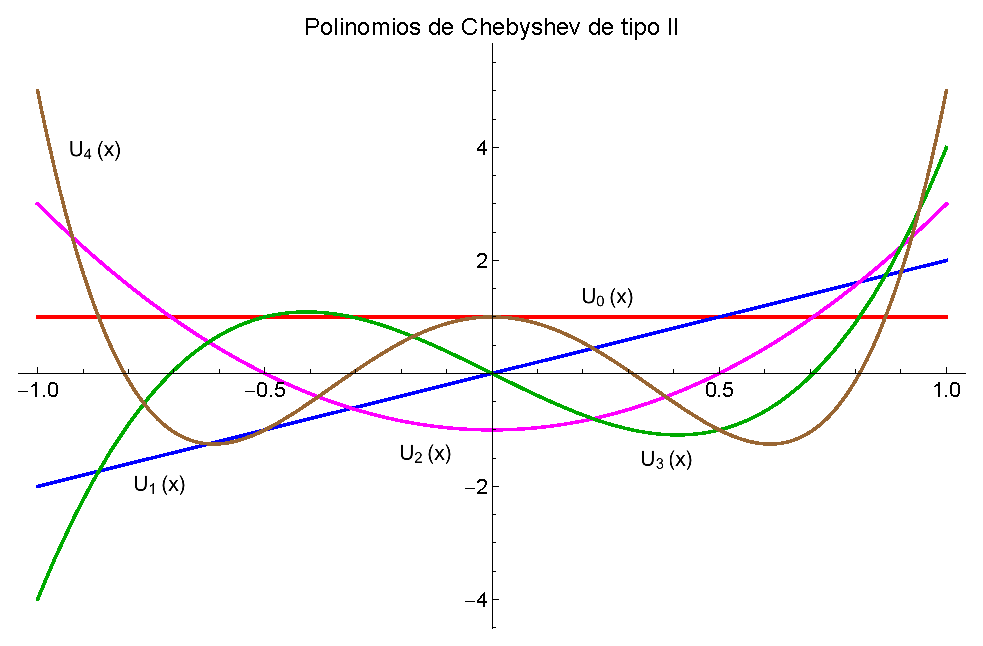
\includegraphics[scale=0.62]{Imagenes/Gram_Schmidt_Chebyshev_2.eps}
\end{figure}
\end{frame}

\end{document}